\begin{figure}[h!]
    \centering
    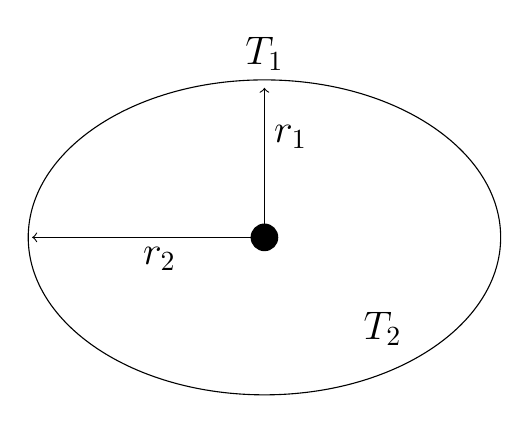
\begin{tikzpicture}
        \fill 
            (0,0) circle (5pt);
        \draw 
            (0,0) ellipse (3cm and 2cm);
        \draw 
            [->, black] (0,0)--(0,1.9);
        \draw 
            [->, black] (0,0)--(-2.95,0);
        \draw 
            (0,1) node[anchor= south west]{\Large$r_{1}$};
        \draw 
            (-1, 0) node[anchor= north east]{\Large$r_{2}$};
        \draw 
            (0,2) node[anchor= south]{\Large$T_{1}$};
        \draw 
            (1.5,-1.5) node[anchor= south]{\Large$T_{2}$};
    \end{tikzpicture}
    \caption{The effect of rotation on a spherically symmetric object. Symmetry is broken and gradients arise.}
    \label{fig:ellipse}
\end{figure}